% Lecture Template for ME3050-001-002-Tristan Hill - Spring 2020 - Summer 2020
% Dynamics Modeling and Controls
% Higher Order Systems - Modeul 13 - Topic 4

% I am finally converting my stuff to BEAMER

% Document settings

%\documentclass{beamer}                  % for presentation ?
\documentclass[handout]{beamer}  % for handout ?
\usepackage{beamerthemesplit}
\usepackage{amsmath}
\usepackage{listings}
\usepackage{multicol}
\usepackage{framed}

\usepackage{amsmath, nccmath}
\usepackage{geometry}
\usepackage{bm}


\beamertemplateballitem

\definecolor{TTUpurple}{rgb}{0.3098, 0.1607, 0.5176} % TTU Purple (primary)
\definecolor{TTUgold}{rgb}{1.0000, 0.8666, 0.0000} % TTU Gold (primary)

\setbeamercolor{palette primary}{bg=TTUpurple,fg=TTUgold}
\setbeamercolor{palette secondary}{bg=black,fg=TTUgold}
\setbeamercolor{palette tertiary}{bg=black,fg=TTUpurple}
\setbeamercolor{palette quaternary}{bg=TTUgold,fg=black}
\setbeamercolor{structure}{fg=TTUpurple} % itemize, enumerate, etc
\setbeamercolor{section in toc}{fg=TTUpurple} % TOC sections

% custom colors
\definecolor{TTUpurple}{rgb}{0.3098, 0.1607, 0.5176} % TTU Purple (primary)
\definecolor{TTUgold}{rgb}{1.0000, 0.8666, 0.0000} % TTU Gold (primary) 
\definecolor{mygray}{rgb}{.6, .6, .6}
\definecolor{mypurple}{rgb}{0.6,0.1961,0.8}
\definecolor{mybrown}{rgb}{0.5451,0.2706,0.0745}
\definecolor{mygreen}{rgb}{0, .39, 0}
\definecolor{mypink}{rgb}{0.9960, 0, 0.9960}

% color commands
\newcommand{\R}{\color{red}}
\newcommand{\B}{\color{blue}}
\newcommand{\BR}{\color{mybrown}}
\newcommand{\K}{\color{black}}
\newcommand{\G}{\color{mygreen}}
\newcommand{\PR}{\color{mypurple}}
\newcommand{\PN}{\color{mypink}}
\newcommand{\OR}{\color{TTU}}
\newcommand{\GD}{\color{TTUgold}}

\newcommand{\Lagr}{\mathcal{L}} % lagrangian

\newcommand{\hspcu}{\underline{\hspace{20mm}}} % large horizontal space w underline
\newcommand{\vspccc}{\vspace{6mm}\\} % large vertical space
\newcommand{\vspcc}{\vspace{4mm}\\}   % medium vertical space
\newcommand{\vspc}{\vspace{2mm}\\}     % small vertical space

\newcommand{\hspcccc}{\hspace{10mm}} % large horizontal space
\newcommand{\hspccc}{\hspace{6mm}} % large horizontal space
\newcommand{\hspcc}{\hspace{4mm}}   % medium horizontal space
\newcommand{\hspc}{\hspace{2mm}}     % small horizontal space

\newsavebox{\mybox} % custom box

\newcommand{\MNUM}{13\hspace{2mm}} % Module number
\newcommand{\TNUM}{4\hspace{2mm}} % Topic number 
\newcommand{\moduletitle}{Higher Order Systems} % Titles and Stuff
\newcommand{\topictitle}{MATLAB Simulation} 

\newcommand{\sectiontitleI}{Control Systems Toolbox} % More Titles and Stuff
\newcommand{\sectiontitleII}{SS function and Dynamic System Object}
\newcommand{\sectiontitleIII}{Step, and Impulse Function}
\newcommand{\sectiontitleIV}{Example: 1DOF Simulation}

\author{ME3050 - Dynamics Modeling and Controls}
\title{Module \MNUM - \moduletitle}
\date{Mechanical Engineering\vspc Tennessee Technological University}

\begin{document}

\lstset{language=MATLAB,basicstyle=\ttfamily\small,showstringspaces=false}

\frame{\titlepage \center\begin{framed}\Large \textbf{Topic \TNUM - \topictitle}\end{framed} \vspace{5mm}}

% Section 0 - Outline
\frame{
	
	\large \textbf{Topic \TNUM - \topictitle} \vspace{3mm}\\
	
	\begin{itemize}
	
		\item \sectiontitleI    \vspc % Section I
		\item \sectiontitleII 	\vspc % Section II
		\item \sectiontitleIII 	\vspc %Section III
		\item \sectiontitleIV 	\vspc %Section IV
	
	\end{itemize}

}


\section{\sectiontitleI}

\frame{
  \frametitle{\sectiontitleI}

Control System Toolbox provides algorithms and apps for systematically analyzing, designing, and tuning linear control systems. You can specify your system as a transfer function, state-space, zero-pole-gain, or frequency-response model. \vspcc

It may have been included when you installed MATLAB but if is it not you can easily install it using the add-ins manager in the home tab.

}


\frame{  
  \frametitle{\sectiontitleI}

	Some Toolbox Functions (\href{ https://www.mathworks.com/help/control/referencelist.html?type=function&listtype=cat&category=index&blocktype=all&capability=}{full list})
	\begin{itemize}
		\item ss
		\item tf
		\item pid
		\item initial
		\item step
		\item impulse
	\end{itemize}

\vspace{5mm}The Toolbox also contains specialized blocks for Simulink

}


\section{\sectiontitleII}

\frame[containsverbatim]{
\frametitle{\sectiontitleII}

Create a dynamic system object with the {\bf ss()} function\vspc

\begin{framed}
\begin{lstlisting}
[Y,T]=step(SYS,TSPAN,OPTIONS)
\end{lstlisting}
\end{framed}

	\begin{itemize}

		\item \underline{Input 1:} SYS - dynamic system object\vspc
		\item \underline{Input 2:} TSPAN - array of time values for simulation  \vspc
		\item \underline{Input 3:} OPTIONS - created by stepDataOptions function \vspc
		\item \underline{Output 1:} Y - simulation response as array \vspc
		\item \underline{Output 2:} T - simulation time as array\vspc

	\end{itemize}

}


\frame{  
  \frametitle{\sectiontitleII}

	SYS - dynamic system object 
	
	\vspace{40mm}


}

\section{\sectiontitleIII}

\frame[containsverbatim]{
\frametitle{\sectiontitleIII}

Simulate the step response of dynamic system with the {\bf step()} function\vspc

\begin{framed}
\begin{lstlisting}
[Y,T]=step(SYS,TSPAN,OPTIONS)
\end{lstlisting}
\end{framed}

	\begin{itemize}

		\item \underline{Input 1:} SYS - dynamic system object\vspc
		\item \underline{Input 2:} TSPAN - array of time values for simulation  \vspc
		\item \underline{Input 3:} OPTIONS - created by stepDataOptions function \vspc
		\item \underline{Output 1:} Y - simulation response as array \vspc
		\item \underline{Output 2:} T - simulation time as array\vspc

	\end{itemize}

}

\frame[containsverbatim]{
\frametitle{\sectiontitleIII}

Simulate the step response of dynamic system with the {\bf step()} function\vspc

\begin{framed}
\begin{lstlisting}
[Y,T]=impulse(SYS,TSPAN)
\end{lstlisting}
\end{framed}

	\begin{itemize}

		\item \underline{Input 1:} SYS - dynamic system object\vspc
		\item \underline{Input 2:} TSPAN - array of time values for simulation  \vspc
		 - use IMPULSEPLOT for more options 
		\item \underline{Output 1:} Y - simulation response as array \vspc
		\item \underline{Output 2:} T - simulation time as array\vspc

	\end{itemize}

}

\section{\sectiontitleIV}

\frame{
	\frametitle{\sectiontitleIV}
		Consider the 1DOF Quarter-Car model with displacement input from the profile of the road.\vspc
	
	\begin{multicols}{2}
		
	
		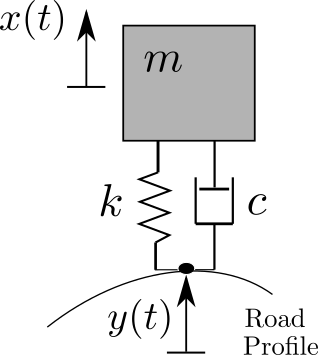
\includegraphics[scale=.4]{quarter_car_1dof_02.png} \vspc
		The standard EOM becomes:
		\[ m\ddot{x} +c(\dot{x}-\dot{y})+k(x-y)=0 \]
	
		The second order EOM can be decomposed into a system of first order differential equations and written as a state space model. \vspc
	
	\end{multicols}

}


\frame{  
	\frametitle{\sectiontitleIV}
	The displacement input requires a {\it clever} substitution.  
 	\begin{fleqn}
		\[ m\ddot{x}+c(\dot{x}-\dot{y})+k(x-y)=0 \] 
		\[ z_1=x \hspc and \hspc z_2=\dot{x}-\frac{c}{m}y \]
		\[ \dot{z}_2=-\frac{c}{m}(z_2+\frac{c}{m}y)-\frac{k}{m}z_1+\frac{k}{m}y \hspc and \hspc \dot{z}_1=z_2+\frac{c}{m}y \] 
	\end{fleqn}
	
	Finally, write the state equation.
	\[
	\begin{bmatrix}
	\dot{z}_{1} \vspace{3mm}\\
	\dot{z}_{2}
	\end{bmatrix}
	=
	\begin{bmatrix}
	0& 1\vspace{3mm}\\
	-\frac{k}{m} & -\frac{c}{m}
	\end{bmatrix}
	\begin{bmatrix}
	z_1\vspace{3mm}\\
	z_2
	\end{bmatrix}
	+
	\begin{bmatrix}
	\frac{c}{m}\vspace{3mm}\\
	-(\frac{c}{m})^2+\frac{k}{m}
	\end{bmatrix}
	y(t)
	\]
}

\frame{
\frametitle{\sectiontitleIV}
It is important that you keep the same substitutions when writing the output equations.\vspc

Output 1 - Position:\hspc $ y_{O1}=x=z_1 $\vspc

Output 2 - Velocity:\hspc $ y_{O2}=\dot{x}=\dot{z}_1=z_2+\frac{c}{m}y $\vspc

\[
\begin{bmatrix}
\dot{y}_{O1} \vspace{3mm}\\
\dot{z}_{O2}
\end{bmatrix}
=
\begin{bmatrix}
1& 0\vspace{3mm}\\
0 & 1
\end{bmatrix}
\begin{bmatrix}
z_1\vspace{3mm}\\
z_2
\end{bmatrix}
+
\begin{bmatrix}
0\vspace{3mm}\\
\frac{c}{m}
\end{bmatrix}
y(t)
\]

}

% references is not a section for now, for looks and it would be a waste of space
\frame{

\frametitle{References}

\begin{itemize}
	\item System Dynamics, Palm III, Third Edition -
	\item MATLAB-State Space handout - FIX TYPO IN HANDOUT!
\end{itemize}

}
\end{document}









